\section{Edifici}
\subsection{Ricerca di un edificio}
Da questa schermata l'utente può provare a cercare edifici intorno a sè. \\ Cliccando il \gl{checkbox} ``Ricerca per raggio'' e poi muovendo lo \gl{slider} sottostante può decidere in che raggio di distanza cercare edifici. Una volta cliccato il pulsante ``CERCA EDIFICI NEL RAGGIO SELEZIONATO'' compariranno al di sotto dello stesso bottone la lista degli edifici presenti nel raggio selezionato. \\ 
Successivamemte basterà cliccare sull'edificio desiderato per accedere alla schermata in cui vengono visualizzate informazioni riguardo l'edificio e i percorsi disponibili nell'edificio stesso.
\begin{figure}[!h]
	\centering
	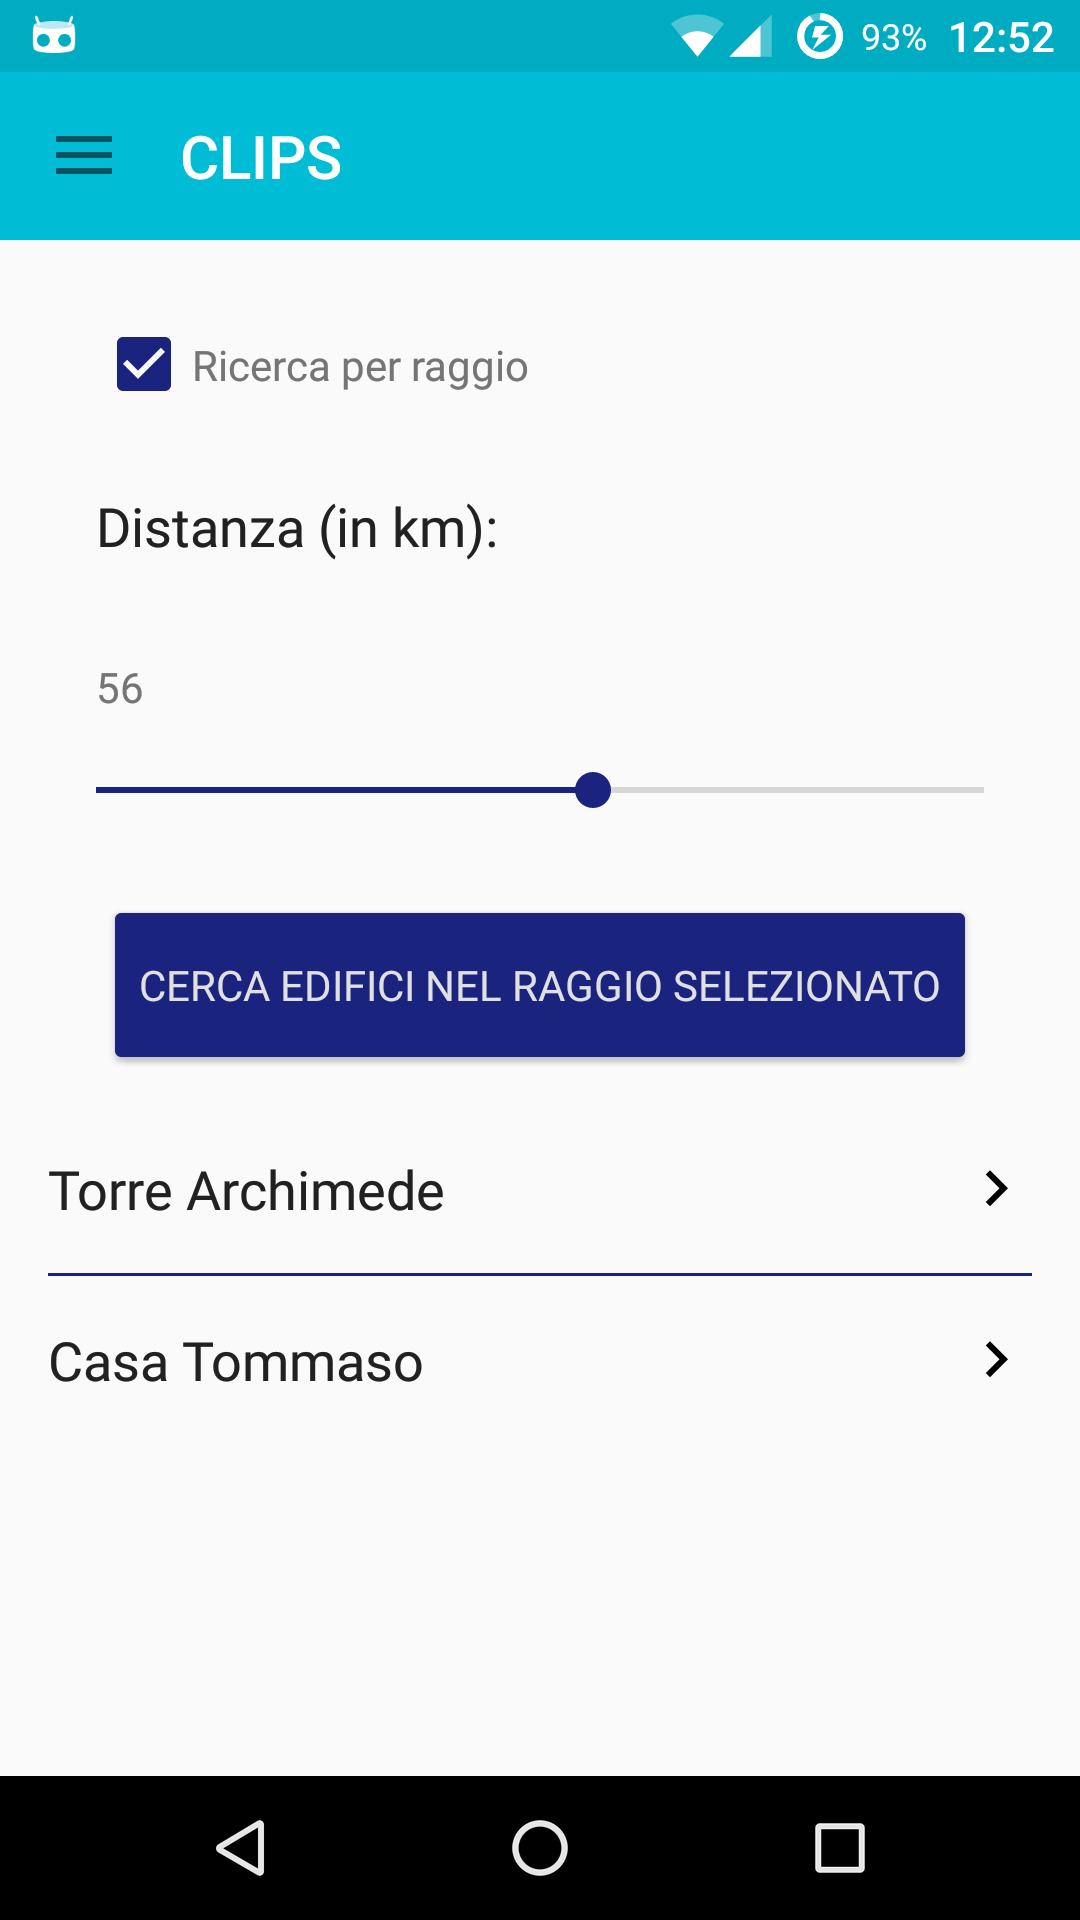
\includegraphics[scale=0.15]{screenshot/searchedifici}
	\caption{Schermata di ricerca edifici}
\end{figure}

\begin{figure}[!h]
	\centering
	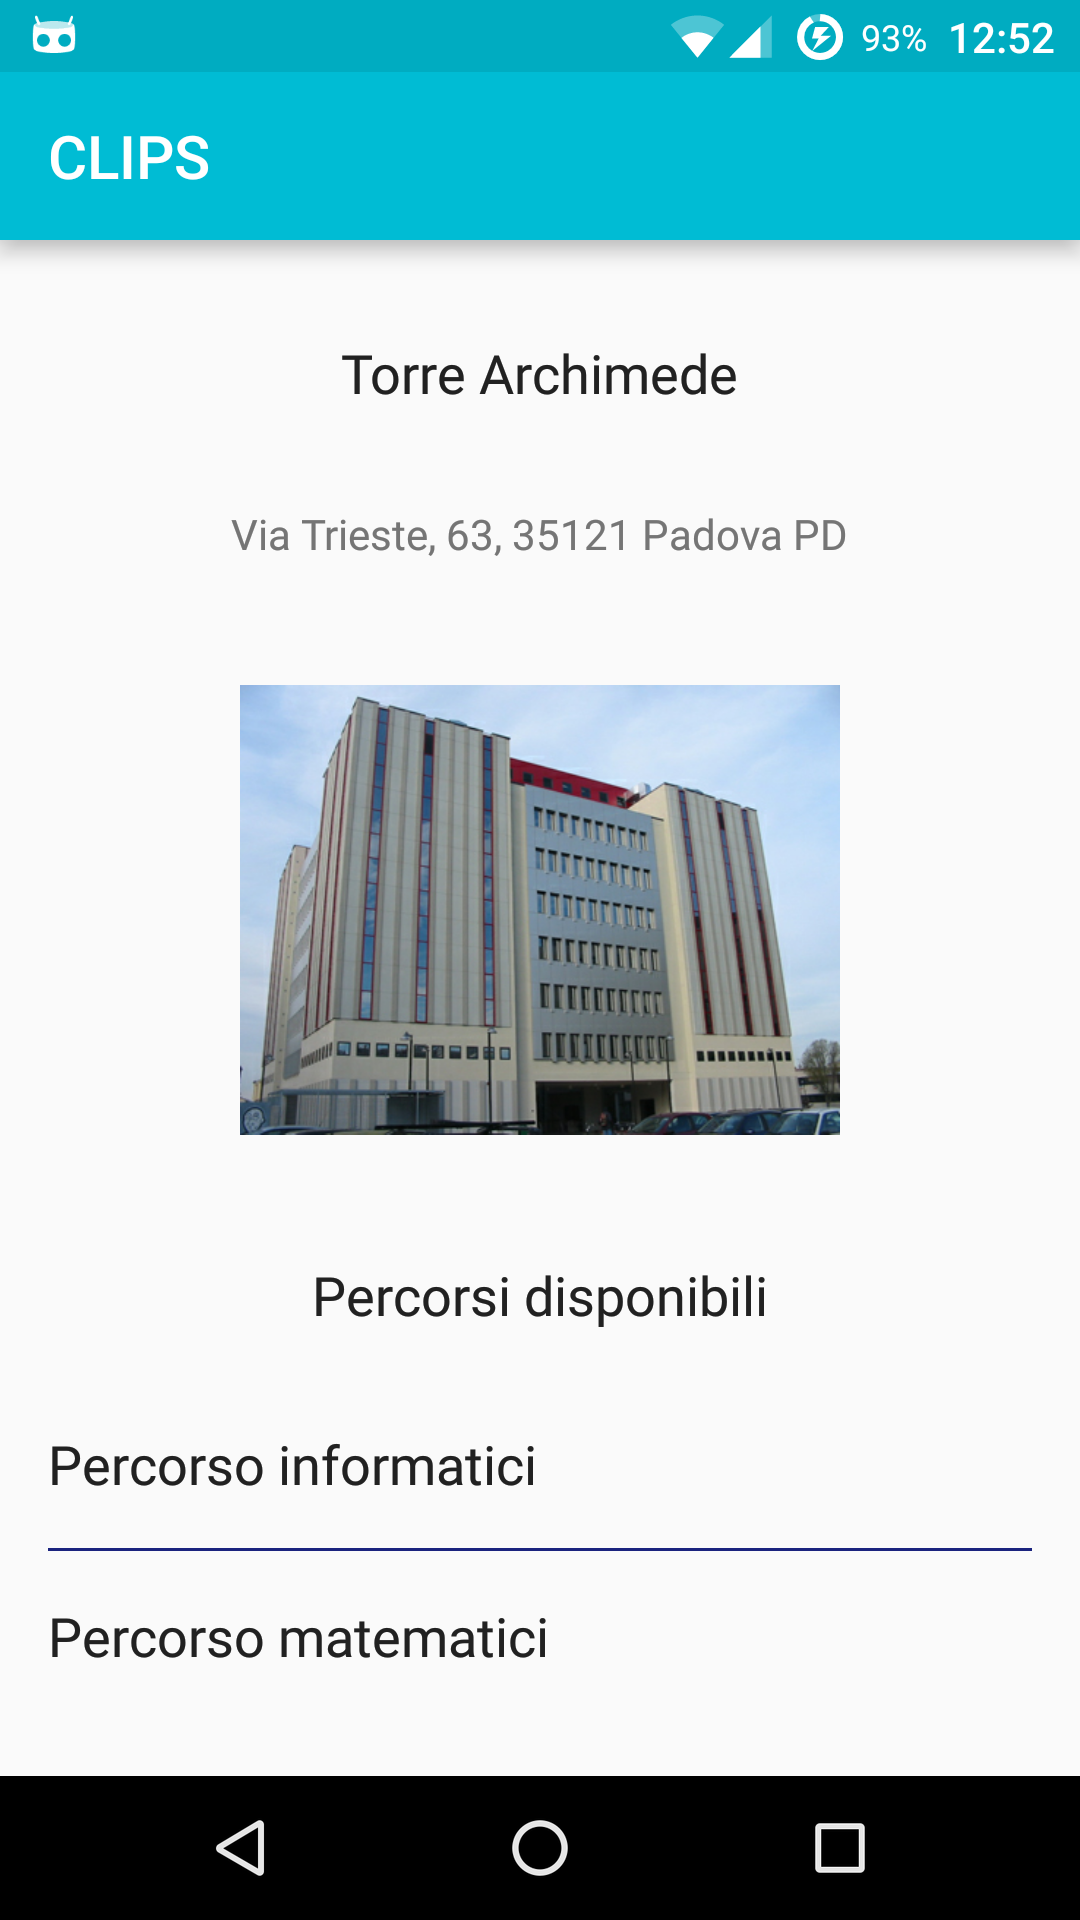
\includegraphics[scale=0.15]{screenshot/edificio}
	\caption{Schermata di dettaglio edificio}
\end{figure}